
\chapter{BUILDING PAGE OBJECTS FOR HUBCHECK}
\label{chap:page_objects}

% 2. building page objects
%    |- breaking web pages into widgets
%    |- matching web page widgets to HUBcheck widgets
%    |- building new widgets
%    |- new page object design patterns
%       |- iframewrap pattern
%       |- list-row pattern
%       |- form pattern

The Page Object design pattern is the cornerstone in creating compact easy to
read automation scripts, and it is key in combating brittle test cases. The
pattern uses object methods to represent the services offered on a web page. By
doing this, the pattern encourages automation developers to move the low level
details of how a task is completed out of automation scripts and into
libraries. This leaves the automation script with abstract generalizations of
what should happen and calls to the library that make those generalizations
happen.

In this chapter, we briefly review why the Page Object design pattern is
important, dive into how to use HUBcheck's page objects, and learn how to build
new page objects that work with the HUBcheck library. We'll also investigate
three new design patterns that are helpful when building page objects for
HUBcheck.

\section{Review of the Page Object Design Pattern}
\label{sec:review_page_object_design_pattern}

\begin{xcode}{%
  language=Python,%
  label=lst:hubzero_login_without_pageobjects,%
  caption={Login automation script for hubzero.org}%
}
from selenium import webdriver

# start the browser and navigate to the login page
browser = webdriver.Firefox()
browser.get('https://hubzero.org/login')

# perform the login action
browser.find_element_by_css_selector("#username").clear()
browser.find_element_by_css_selector("#username").send_keys("testuser")
browser.find_element_by_css_selector("#passwd").clear()
browser.find_element_by_css_selector("#passwd").send_keys("abc123")
browser.find_element_by_css_selector("[name='Submit']").click()
\end{xcode}

In \Cref{ssec:external_libs_selenium_page_objects}, we first introduced an
automation script that performed a user login on a hub, noting a few
undesirable patterns within the script. First we identified repetition in
searching for the username and password fields. Second we noted the pattern of
clearing the field before sending data to it. While it isn't always necessary
to clear an input before sending data to it, this tends to be good practice
that helps remove previously set values from fields.  One pattern we didn't
note has to do with the login action on a larger scale.  The action as a whole
takes about five lines of code to populate the username field, populate the
password field, and click the login button. The problem arises when the login
service is used in multiple scripts.  Writing these five lines of code over and
over is costly and is prone to variation. Furthermore, it adds to the
brittleness of all of the automation scripts.

Consider the case where the developer would like to use a set of automation
scripts, with these five lines of login code, on another hub website, like
nanohub.org.  The developer may find that while the scripts worked on
hubzero.org, things are a little different on nanohub.org. In particular, the
element locators for the password input field and login button on hubzero.org
don't match the ones on nanohub.org. On hubzero.org, the password input field
is identified by the css selector \xflocator{\#passwd}, while on nanohub.org,
the same field is identified by the css selector \xflocator{\#password}.
Similarly, on hubzero the login button is identified by the css selector
\xflocator{[name=`Submit']}, while on nanohub.org it is identified by the css
selector \xflocator{\#login-submit}.

\begin{figure}[ht!]
        \centering
        \begin{subfigure}[b]{0.4\textwidth}
                \centering
                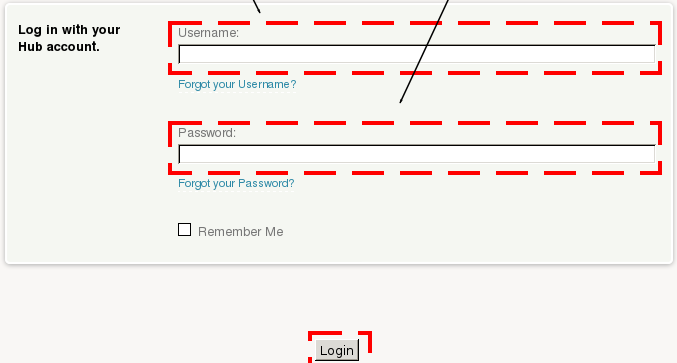
\includegraphics[width=\textwidth]
                  {../../images/hubzero_login_form_with_locators.png}
                \caption{ hubzero.org login form. }
                \label{fig:login_form_with_locators_hubzero}
        \end{subfigure}
        \begin{subfigure}[b]{0.4\textwidth}
                \centering
                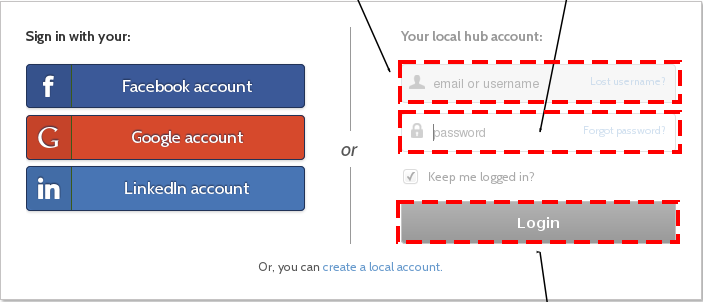
\includegraphics[width=\textwidth]
                  {../../images/nanohub_login_form_with_locators.png}
                \caption{ nanohub.org login form. }
                \label{fig:login_form_with_locators_nanohub}
        \end{subfigure}
        \caption{The variation in locators used on the hub login page causes an
                 additional level of complexity when trying to develop automation
                 scripts generic enough to work across the hubs managed by the
                 HUBzero team.}
        \label{fig:login_form_locators}
\end{figure}

With every new hub the automation script is taken to, there is the opportunity
for either of the previous element locator sets to be used, or even a new set.
Keeping separate automation scripts for each hub is a good way to encourage
divergence of the source. Instead the script should be written in a way where
the differences are abstracted away. This is one of the goals of the Page
Object design pattern.

\begin{xcode}{%
  language=Python,%
  label=lst:login_page_pageobject,%
  caption={Page object for the hub /login page}%
}
# pageobjects.py
locdict = {
  'hubzero' : {
    'username' : '#username',
    'password' : '#passwd',
    'login_b'  : "[name='Submit']"
  },
  'nanohub' : {
    'username' : '#username',
    'password' : '#password',
    'login_b'  : '#login-submit'
  }
}

class LoginPage(object):
    def __init__(self,browser,hub):
        self.username = \
            browser.find_element_by_css_selector(locdict[hub]['username'])
        self.password = \
            browser.find_element_by_css_selector(locdict[hub]['password'])
        self.login_b = \
            browser.find_element_by_css_selector(locdict[hub]['login_b'])

    def login_as(self,username,password):
        self.username.clear().send_keys(username)
        self.password.clear().send_keys(password)
        self.login_b.click()
\end{xcode}

\Cref{lst:login_page_pageobject} shows an example page object for the
hub login page that can be configured to work with hubzero.org or nanohub.org.
The \xfparameter{locdict} variable holds dictionaries of locators that are used by
the \xfclass{LoginPage} class. The user specifies which hub locators they want
to use in the \xfclass{LoginPage} constructor.


\begin{xcode}{%
  language=Python,%
  label=lst:hubzero_login_with_pageobjects,%
  caption={Login automation script for hubzero.org, using page objects}%
}
from selenium import webdriver
from pageobjects import LoginPage

# start the browser and navigate to the login page
browser = webdriver.Firefox()
browser.get('https://hubzero.org/login')

# perform the login action
po = LoginPage(browser,hub='hubzero')
po.login_as(username="testuser",password="abc123")
\end{xcode}


In line 9 of \Cref{lst:hubzero_login_with_pageobjects}, the page object
is created and configured to use the \xflocfam{hubzero} locators. Next, the
automation script calls the page object's \xfmethod{login\_as()} method to
perform the login service on the page.

The page object solution is flexible and robust, allowing the developer to
update the page object to handle more hubs by adding locators to the
\xfparameter{locdict} variable. The new automation script can easily be configured
to work on nanohub.org, or any other hub recognized by the page object.
Additionally, all of the code to perform the login action is in one place, the
\xfmethod{login\_as()} method. If there is a change to how the login service
works, an update to the \xfmethod{login\_as()} method updates all of the scripts
that use the method. The HUBcheck library provides classes for popular HTML
elements to help developers quickly build page objects. Let's explore how to
rebuild the LoginPage page object by using the HUBcheck library.



\section{Rebuilding the Login Page Object With HUBcheck}
\label{sec:rebuilding_login_page_object_with_hubcheck}
% web pages can be thought of as elements and actions
% elements are the pieces you would like to interact with
% actions are the services the web page can perform for you.
% actions are generally a collection of interactions with elements.
% consider the hub login page.
% The hub login page has 



%HUBcheck page objects build upon the idea of dynamically loading page objects
%as a part of the object's configuration. While the HUBzero team supports over
%twenty hubs, the hub configurations can be narrowed down to about three or four
%sets of locators for most page objects. The majority of the variation in
%locators is due to hub software versioning or template differences between
%hubs.
%
%\subsubsection{HUBcheck Page Object base classes}
%
%HUBcheck provides two base classes for creating page objects, the
%\textit{BasePageObject} class and the \textit{BasePageWidget} class. New page
%object classes can be derived from the \textit{BasePageObject} class and
%constructed by combining together multiple \textit{BasePageWidget} objects.
%The \textit{BasePageObject} class allows developers to provide an API for the
%services available on a web page, while the incorporated
%\textit{BasePageWidget} classes perform the work of completing the actions
%associated with the services.
%
%% FIXME: need to add info on what the BasePageObject and BasePageWidget classes
%% are BasePageObject is a container for BasePageWidgets
%
%\subsubsection{Building a Page Object using the BasePageWidget class}

Before representing a web page as a page object, the developer must understand
the purpose of the web page.  Web pages provide services. When a user navigates
to a web page, they are either receiving information from the system
or providing information to the system.  On the hub, the login web page provides
four services. The most recognized service is providing user authentication for
accessing personalized and restricted material on the hub. The other services
provided by the page are to guide users to the registration page, the username
reminder page, and the password reset page.

\begin{figure}[tbh]
  \centering
  \includegraphics[width=0.75\textwidth]
    {../../images/annotated/hubzero_login_page_parts.png}
  \caption{ The part of the web page represented by the Login widget is outlined in red. }
  \label{fig:hubzero_login_page_parts}
\end{figure}

The login web page can be split into three sections. The header section is the
top portion of the page available on all hub web pages. This includes site
navigation links and banners. The footer section is the bottom portion of the
page, also available on all hub web pages. This section includes copyright,
contact, and site ownership information. The rest of the page can be considered
the Login widget, and is shown in \Cref{fig:hubzero_login_page_parts}.
The Login widget is a mega widget, a widget made up of smaller widgets or
elements, like links, text boxes, checkboxes, and buttons. Each of these elements
are widgets in their own right, and the classes that represent them provide a
few specialized services.

\subsection{Matching Web Page Widgets to HUBcheck Page Object Classes}
\label{ssec:matching_widgets_to_page_objects}

\begin{figure}
        \centering
        \begin{subfigure}[b]{0.5\textwidth}
                \centering
                \includegraphics[width=\textwidth]{../../images/annotated/hubzero_login_page_textbox.png}
                \caption{Text box widgets}
                \label{fig:login_page_text_boxes}
        \end{subfigure}
        \begin{subfigure}[b]{0.5\textwidth}
                \centering
                \includegraphics[width=\textwidth]{../../images/annotated/hubzero_login_page_links.png}
                \caption{Link widgets}
                \label{fig:login_page_links}
        \end{subfigure}
        \begin{subfigure}[b]{0.5\textwidth}
                \centering
                \includegraphics[width=\textwidth]{../../images/annotated/hubzero_login_page_cb_button.png}
                \caption{Checkbox and Button widgets}
                \label{fig:login_page_cb_button}
        \end{subfigure}
        \caption{The login web page is made up of several types of widgets.}
        \label{fig:login_page_widgets}
\end{figure}

On the login page, each element can be represented by a HUBcheck page object
class. Links are represented by the \xfclass{Link} class, input text boxes are
represented by the \xfclass{Text} class, checkboxes are represented by the
\xfclass{Checkbox} class, and buttons are represented by the \xfclass{Button}
class.  \Cref{lst:login_page_data_members} starts to build a new
\xfobject{Login} page object by identifying the widgets that are available on
the web page and matching them up with comparable HUBcheck classes.  In the
code, the username and password text boxes are represented by \xfobject{Text}
objects. The username reminder, password reset, and register links are
represented by \xfobject{Link} objects. The remember me checkbox is represented
by a \xfobject{Checkbox} object and the form submission button is represented
by a \xfobject{Button} object.  HUBcheck includes nine classes that represent
popular HTML elements including \xfclass{Button}, \xfclass{Checkbox},
\xfclass{Link}, \xfclass{Radio}, \xfclass{Select}, \xfclass{Text},
\xfclass{TextReadOnly}, \xfclass{TextAC}, \xfclass{TextArea}, and
\xfclass{Upload}.

\begin{xcode}{%
  language=Python,%
  label=lst:login_page_data_members,%
  caption={The Login class is a composition of other classes representing the %
           elements on the web page.}%
}
class Login(BasePageWidget):
    def __init__(self):
        ...
        self.username  = Text(self,{'base':'username'})
        self.password  = Text(self,{'base':'password'})
        self.remember  = Checkbox(self,{'base':'remember'})
        self.remind    = Link(self,{'base':'remind'})
        self.reset     = Link(self,{'base':'reset'})
        self.register  = Link(self,{'base':'register'})
        self.submit    = Button(self,{'base':'submit'})
        ...
\end{xcode}

The \xfclass{Login} page object has methods that mirror the services offered by
the login web page. These methods abstract away the steps required to perform
the service and reduce the service to a single call to the page object's API.
\Cref{lst:login_page_member_functions} declares four methods that
correspond to the services provided by the login page, including
\xfmethod{login\_as()}, \xfmethod{goto\_remind()}, \xfmethod{goto\_reset()},
and \xfmethod{goto\_register()}.

\begin{xcode}{%
  language=Python,%
  label=lst:login_page_member_functions,%
  caption={The Login object's methods match the services provided by  %
            the widget.}%
}
class Login(BasePageWidget):
    ...
    def login_as(self,username,password):
        self.username.value = username
        self.password.value = password
        self.submit.click()
    def goto_remind(self):
        self.remind.click()
    def goto_reset(self):
        self.reset.click()
    def goto_register(self):
        self.register.click()
\end{xcode}


Inside the methods, page object data members representing the web page elements
take over to do the real work of typing values into the login form's fields,
clicking links or buttons, and toggling checkboxes. For the
\xfmethod{login\_as()} method, the \xfparameter{self.username} and
\xfparameter{self.password} objects are responsible for updating the username
and password fields on the web page by using the method's arguments as inputs.
\xfparameter{self.username} and \xfparameter{self.password} are both instances
of the \xfclass{Text} class, with a \xfparameter{value} property which acts as
an accessor, allowing users to query or set the current value of the field on
the web page. In line 4 of \Cref{lst:login_page_member_functions},
\xfparameter{self.username}'s \xfparameter{value} property is assigned a new
value. This assignment causes a Selenium WebDriver handle for the text input
field to be retrieved from the web page's HTML DOM.  The text input field is
cleared of any previous value, and the new value is written to the field on the
web page. This happens again, in line 5, for the \xfparameter{self.password}
object. Lines 9 - 12 of \Cref{lst:text_widget_value_property} show the
sequence of events in more detail.

\begin{xcode}{%
  language=Python,%
  label=lst:text_widget_value_property,%
  caption={The Text object manages finding and writing to the Selenium  %
            WebDriver object handle.}%
}
class Text(BasePageWidget):
    @property
    def value(self):
        e = self.owner.find_element_in_owner(self.locator)
        return e.get_attribute('value')

    @value.setter
    def value(self, val):
        e = self.owner.find_element_in_owner(self.locator)
        e.click()
        e.send_keys(Keys.CONTROL,'a')
        e.send_keys(val)
\end{xcode}

\subsection{Specifying Element Locators for Page Object Classes}
\label{ssec:specifying_page_object_element_locators}

The \xfclass{Login} page object is almost complete. In
\Cref{lst:login_page_data_members}, we specified the elements available on the
login web page. In \Cref{lst:login_page_member_functions} we added
functions to fulfill all of the services offered by the web page. The next step
is to specify the locators for the web page elements.

HUBcheck page object classes have a complementary set of
locator classes that specify sets of element
locators. \Cref{lst:login_page_object_locators} shows two example
locator classes for the hubzero.org and nanohub.org login pages discussed in
\Cref{sec:review_page_object_design_pattern}.

\begin{xcode}{%
  language=Python,%
  label=lst:login_page_object_locators,%
  caption={Locators for the Login page object}%
}
class Login_Locators_Base_1(object):
    locators = {
        'username'  : "css=#username",
        'password'  : "css=#passwd",
        'submit'    : "css=[name='Submit']",
        ...
    }

class Login_Locators_Base_2(object):
    locators = {
        'username'  : "css=#username",
        'password'  : "css=#password",
        'submit'    : "css=#login-submit",
        ...
    }
\end{xcode}

Each locator class holds a dictionary of locators that is dynamically loaded by
the page object class during initialization and is used to override the
locators of its data members.  In \Cref{lst:login_page_data_members},
the \xfparameter{self.submit} data member is instantiated with the dictionary
\xfinlinecode{\{`base': `submit'\}} as one of the arguments. This is a locator
override, which maps the \xfinlinecode{`base'} locator inside of the
\xfparameter{self.submit} object to the value of the \xfinlinecode{`submit'} locator of
the \xfclass{Login} page object. The value of the \xfinlinecode{`submit'} locators is
dynamic because it depends upon which locator class is loaded by the page
object, \xfclass{Login\_Locators\_Base\_1} or \xfclass{Login\_Locators\_Base\_2}.

The pattern of separating locators from the page object allows HUBcheck page
objects to be used across multiple hubs. When new hubs are created new locators
can be added to the system, if needed, leaving the page object classes
untouched. More often then not, new hubs use locators that have already been
added to the HUBcheck library.  When new versions of the HUBzero software are
released, the locators also can be added to the HUBcheck library without
modifying the existing page objects. In the next section, we dive deeper into
patterns that can be used to build page objects. While these patterns can be
found throughout the HUBcheck library, they include ideas that are best
practices for building all kinds of page objects.


\section{Incorporating Classic Design Patterns into Page Objects}
\label{sec:incorporate_design_patterns_into_page_objects}

The social aspect of the hub website encourages members to contribute content
and organize in communities. To do this, the user must interact with hub web
pages containing web forms, evaluate search results represented as lists or tables,
and upload content. These three forms of interaction often show up in the web
components built for the hub, and by extension, in the page objects built to
interface with those web components.

For most web pages, identifying the widgets and services for the page is
straight forward. For other web pages, the widgets are not so obvious and
inefficient solutions can lead to bad interfaces that add work for developers
instead of reducing work. Three types of interactions found on the hub fall
into this latter group of web pages: using web forms, reading lists
of data, and interacting with items in iframes.

In this section, we'll introduce three patterns, the WebForm pattern,
the ItemList pattern, and the IframeWrap pattern, that can be
used to quickly produce page objects that work with components that ask the
user to interact through web forms, lists of items, or through an iframe.


\subsection{WebForm Pattern}
\label{ssec:webform_pattern}

Web forms are ubiquitous across the web. They are the best way to collect
information from the user, so there is no wonder why they are a part of many
hub web components. On the hub, users experience them as a part of larger
processes to create, update, or delete content. Interacting with most web forms
takes place in two phases, population and submission.  The first phase,
populating the form, involves searching for fields in the form and assigning
them values. The second phase, submitting the form, simply involves clicking
the submit button on the form.

Many of the harder to test aspects of a hub's web site involve working through
multi-step processes that often include web forms. The novice approach to
creating page objects for these web forms can lead to unintuitive interfaces.
The hub login page and new support ticket page are classic examples of web
forms. When evaluated separately, the interfaces may seem very different.
Certainly the services provided by the pages are different and so are the
fields that need to be populated, but these things can be considered
configuration steps for a class that tackles the larger problem of form
population and submission.

\begin{figure}[tbh]
  \centering
  \includegraphics[width=0.75\textwidth]
    {../../images/hubzero_dropdown_support_ticket_form.png}
  \caption{ Testing the hubzero.org support ticket form. }
  \label{fig:hubzero_dropdown_support_ticket_form}
\end{figure}

% show the support ticket page
% explain that usual way to interact with the support ticket page is to
% create a page object with a bunch of accessor methods for setting fields
% on the web page. the last thing to do is click the submit button.
% this approach makes the developer have to lookup all of the accessor methods
% for the page object and makes reading the inputs for the form hard to read.
% the proposed interface stores the 


\begin{xcode}{%
  language=Python,%
  label=lst:trouble_report_form_po_interface_1,%
  caption={The typical interface for a web form requires the automation %
           developer to call page object accessors to populate the form.}%
}
po = TroubleReportForm()

po.set_name('testuser')
po.set_email('tu@hubzero.org')
po.set_problem('test problem')
po.set_upload('myscreen.png')

po.submit.click()
\end{xcode}

The typical page object interface for a web form requires the automation
developer to call page object accessor methods to populate each field of a
form. Using accessor methods provides a clean interface for the populate phase.
An alternative approach is to pass the form inputs to a single method, and
allow the method to perform the form population. Similarly, for submitting a
web form, a single method can be used to populate and submit the form. This is
the idea behind the WebForm pattern.
\Cref{lst:trouble_report_form_po_interface_2} shows an example of the interface.


%  caption={The proposed interface for a web form utilizes two methods,
%           \textit\{populate\_form()\} to handle filling in the form inputs,
%           and \textit\{submit\_form()\} to handle form submission.}%
\begin{xcode}{%
  language=Python,%
  label=lst:trouble_report_form_po_interface_2,%
  caption={An example interface for a web form utilizing two methods, %
           populate\_form() to handle filling in the form inputs, %
           and submit\_form() to handle form submission.}%
}
po = TroubleReportForm()

data = {
  'name'    : 'testuser',
  'email'   : 'tu@hubzero.org',
  'problem' : 'test problem',
  'upload'  : 'myscreen.png'
}

po.populate_form(data)

po.submit_form()
\end{xcode}


The purpose of the WebForm pattern is to help standardize the interface for
filling out web forms.  The usual interface makes the script writer work hard
to remember the accessor methods for the inputs on the form. The WebForm
pattern encourages the automation developer to organize the inputs for the form
and send the inputs to a standard page service, the \xfmethod{populate\_form()}
method. Later the user can submit the form using another standard service, the
\xfmethod{submit\_form()} method. These two services are supported for all
forms.

Implementing the WebForm pattern requires a page object that represents a web
form to be derived from an abstract base class that provides the
\xfmethod{populate\_form()} and \xfmethod{submit\_form()} methods.
\Cref{lst:web_form_pattern_formbase} shows an example of such a class.


%While the
%page provides a number of services, the most often used service is the web
%form. The page object from
%\Cref{sec:rebuilding_login_page_object_with_hubcheck} performs both phases the
%population and submission phases of web form interaction in the
%\textit{login\_as()} method, but it could be rewriten to expose these two
%independent actions seperately and provide an easy to read interface that is
%common to all web forms by using the \textit{WebForm} pattern.

%The WebForm pattern provides a standard way to automate the
%interaction with web forms. The class that implements the pattern would need a
%way to accept information regarding the available fields of the web form. The
%two phases can be considered services of the web page, and implemented as
%methods of the class. Page objects could then be derived from this class to get
%the standard interface for a web form. An example class is shown in
%\Cref{lst:web_form_pattern_formbase}.

\begin{xcode}{%
  language=Python,%
  label=lst:web_form_pattern_formbase,%
  caption={\xfclass{FormBase} is an example base class for web forms}%
}
class FormBase(BasePageWidget):
    def __init__(self, owner, locatordict={}):
        ...
        self.submit = Button(self,{'base':'submit'})

    def populate_form(self, data):
        for (k,v) in data:
            widget = getattr(self,k)    # find the widget
            widget.value = v            # set its value

    def submit_form(self,data=[]):
        self.populate_form(data)
        return self.submit.click()
\end{xcode}

In \Cref{lst:web_form_pattern_formbase}, the \xfclass{FormBase} class provides
a submit button object in the constructor, and relies on the derived class to
supply the fields of the form as data members. The two services of the web
form, populating the form and submitting the form, are performed by the class's
\xfmethod{populate\_form()} and \xfmethod{submit\_form()} methods.

\begin{figure}[tbh]
  \centering
  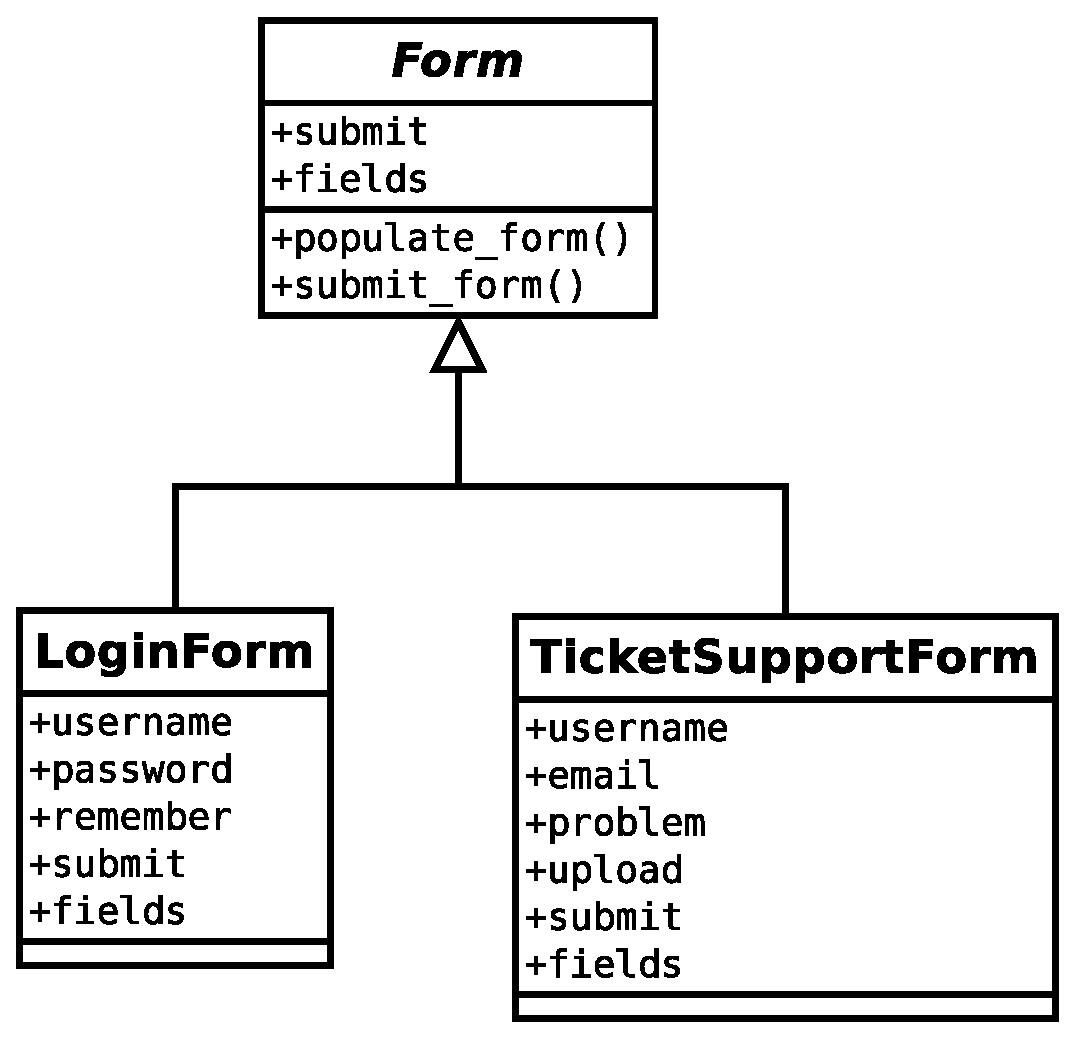
\includegraphics[width=0.50\textwidth]
    {../../diagrams/webform_pattern.png}
  \caption{ In the WebForm pattern, the \xfclass{FormBase} base class
            provides the two services essential to all web forms,
            populating the form and submitting the form. }
  \label{fig:webform_pattern_class_diagram}
\end{figure}

The \xfclass{FormBase} class can be applied to the hub login page example from
\Cref{sec:rebuilding_login_page_object_with_hubcheck} just as easily as it can
be applied to the new support ticket page from
\Cref{fig:hubzero_dropdown_support_ticket_form}, they are both web forms after
all.  To build a new page object for the login page, the first step is to
subclass \xfclass{FormBase} and add the form's fields to the new class's
constructor.  \Cref{lst:web_form_pattern_login_page} shows what the new
page object class would look like.

\begin{xcode}{%
  language=Python,%
  label=lst:web_form_pattern_login_page,%
  caption={An example page object for the hub login page, using \xfclass{FormBase}}%
}
class LoginPage(FormBase):
    def __init__(self, owner, locatordict={}):
        super(LoginPage,self).__init__(owner,locatordict)
        ...
        self.username = Text(self,{'base':'username'})
        self.password = Text(self,{'base':'password'})
        self.remember = Checkbox(self,{'base':'remember'})
\end{xcode}

The new LoginPage class is derived from the FormBase class.  In the LoginPage
constructor, we add data members for the fields of the login page's form, the
username field, the password field, and the remember checkbox. That's it!
Users can interact with the LoginPage page object by supplying the values for
the fields as a dictionary or a list of tuples to either of the inherited
service methods, \xfmethod{populate\_form()} or \xfmethod{submit\_form()}, and
the service methods take care of inspecting the LoginPage object for the
widgets.


\begin{xcode}{%
  language=Python,%
  label=lst:web_form_pattern_using_login_po,%
  caption={Interacting with the new LoginPage page object}%
}
form_data = {'username' : 'testuser',
             'password' : 'abc123',
             'remember' : False}
po = LoginPage()
po.populate_form(form_data.items())
po.submit_form()
\end{xcode}

Using the WebForm pattern simplifies building web form page objects to a single
step of declaring the fields of the form. There are several variations of the
FormBase class, including those that fill out forms in a specified order,
validate inputs, or have extra HTML buttons like cancel or preview. These
variations can usually be accommodated by adjusting the derived class or the
data structures being passed to the base class's service methods.


\subsection{ItemList Pattern}
\label{ssec:itemlist_pattern}

%
% Used to quickly build page objects for web pages that repeatedly list items
% of the same type.
%
% Examples include:
%   1. list of search results.
%   2. table of items.
%
% Real Example: Contribtool Tools Pipeline
%
%

% \subsection{Pattern Name and Classification:}
%
%   ItemList Pattern
%   Purpose: Creational - we are defining a good way to dynamically create
%                         a page object to describe and access a specific
%                         item in a list of items.
%   Scope: Object
%


%\subsection{Intent}

Lists of items on web pages are often built dynamically, pulling information
from databases to present the user with up-to-date information. The
amorphous nature of a web page with a dynamically generated list makes it hard to
build a static page object to represent it. Since the number of items in the
list may fluctuate, it cannot be hard coded into the page object.  Even if it
could, creating individual page objects for each row/item in the list at once
may be memory and time intensive.

Lists of items are an area where the traditional approach to building page
objects is hard to apply. Without knowing ahead of time the number of items in
the list, static page objects cannot be built with an object representing each
item. Instead of manually creating an object for each item in the list, it is
better to step back and evaluate the ways lists are used. Lists are a quick,
organized way of presenting enumerable pieces of data back to the user. Many
lists hold items that provide an overview of the available data by using text
fields or links to web pages with more details. Other types of lists contain
items that exhibit all available data in a single text field. Regardless of the
way the data is displayed, the information in each item depends upon the type
of list being presented.  Users may interact with a single list item at a time
or they may interact with the list as a whole, accessing list properties like
the item count and searching for specific items.

The ItemList design pattern defines a way to dynamically instantiate a page
object that represents a single, specific item from an arbitrarily sized list
of items. Page objects built using this pattern can be used to access the
properties of the single item it was instantiated for and can be quickly
updated to reference another item in the list. The pattern uses elements of the
Iterator pattern \cite{Gamma:1995:DPE:186897} and Factory Method pattern
\cite{Gamma:1995:DPE:186897}, and introduces the concept of the \textit{locator
template}, a template that has a value substituted into it, to create a new web
page element locator.

% FIXME: check out the description and example for the Flyweight pattern
%        to see if it can be applied to the Item class
%
% template locator idea introduced by Adam Goucher


\begin{figure}[ht!]
        \centering
        \begin{subfigure}[b]{0.75\textwidth}
                \centering
                \includegraphics[width=\textwidth]{../../images/hubzero_tool_pipeline_table.png}
        \end{subfigure}
        \begin{subfigure}[b]{0.75\textwidth}
                \centering
                \includegraphics[width=\textwidth]{../../images/hubzero_tool_pipeline_table_html.png}
        \end{subfigure}
        \caption{The hub Tool Pipeline table is a dynamically created list of items.
                 Each row in the table provides links and information regarding a
                 specific simulation tool registered on the hub.}
        \label{fig:itemlist_motivation_tool_pipeline_table}
\end{figure}


In the hub's tool contribution process, the Tool Pipeline, shown in
\Cref{fig:itemlist_motivation_tool_pipeline_table}, is an HTML table that shows
all tools that have been registered on a hub. Each row of the table shows the
tool's title, alias, status, time since the tool was registered, time since the
last status change, and links leading to the tool's resource, status, and
communications history web pages. The Tool Pipeline web page also allows users
to search for specific tools by alias.


Building a page object for a dynamic web page like this is hard because the
information in the table is pulled from a database and may change over time.
While a human user can look at each item quickly to find the item they are
interested in, an automated system must iteratively scan all items until
matching criteria is found. This pattern of listing information from databases
is not unique to the Tool Pipeline page. On the hub, it is also found in the
Tags component when displaying all available tags, in the Support component
when listing support tickets, the Groups component, Questions and Answers,
Projects, Wish List and more.

\begin{figure}[ht!]
        \centering
        \begin{subfigure}[b]{0.45\textwidth}
                \centering
                \includegraphics[width=\textwidth]{../../images/item_list_pattern_container.png}
                \caption{Container class coverage}
                \label{fig:itemlist_container_item_imgs_container}
        \end{subfigure}
        \begin{subfigure}[b]{0.45\textwidth}
                \centering
                \includegraphics[width=\textwidth]{../../images/item_list_pattern_item.png}
                \caption{Item class coverage}
                \label{fig:itemlist_container_item_imgs_item}
        \end{subfigure}
        \caption{The Container and Item classes are the foundation of the ItemList pattern.}
        \label{fig:itemlist_container_item_imgs}
\end{figure}


The ItemList pattern provides a standard way to describe and traverse items in
a list or table on a web page. The main participants of the pattern are two
base classes, \xfclass{Container} and \xfclass{Item}. The container class
represents the meta-data of the list.  Automation developers can ask the
container questions regarding properties of the list, like \textit{how many
items are in the list?} The container cannot answer questions about specific
items in the list, but can provide access to the list elements, either
sequentially or through a limited search capability. The item class represents
a single item in the list.  Automation developers can query this class for
information about the item it represents in the list. Additionally, the item
class can be updated on the fly to point to another item from the list. The
container and item classes provide interfaces that, when implemented, can be
used to represent lists, tables, and other data structures that appear on the web
page as a collection of items.

\begin{figure}[tbh]
  \centering
  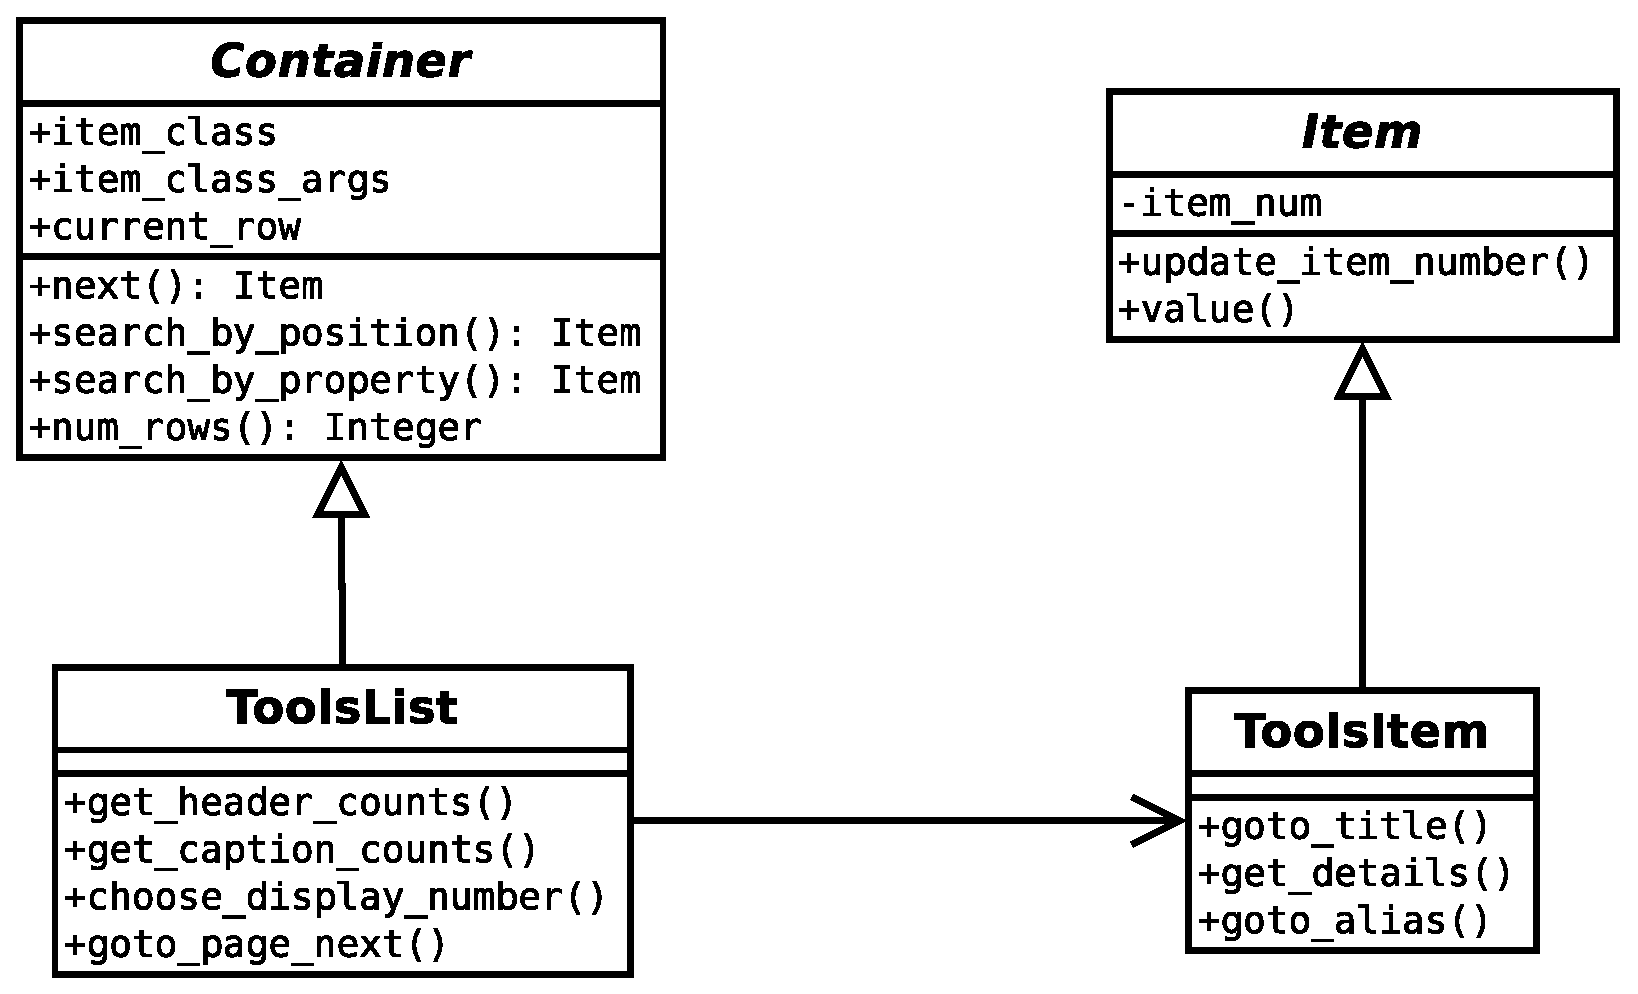
\includegraphics[width=0.75\textwidth]
    {../../diagrams/itemlist_pattern.png}
  \caption{ The ItemList pattern uses a container class to represent the
            list and provide access to list meta-data while providing
            access to elements of the list through an item class. It
            incorporates the Iterator and FactoryMethod patterns. }
  \label{fig:itemlist_pattern_class_diagram}
\end{figure}

%Let's take a closer look at how we can implement a container class. We
%mentioned earlier that the container class should provide access to the list
%meta-data. One of the more frequent queries for the container class asks
%\textit{how many items are in the list?}


%The pattern involves two classes, the Container
%class and the Item class. The Container class describes the properties of the
%list, including decorations like counters that may be at the top or bottom of
%the displayed widget. It also provides ways to access individual items in
%the list which are represented by the Item class. The Item class serves as a
%template for an item in the list. It provides ways to access the properties of
%the specific item in the list that it represents, as well as a way to update
%which item in the list it represents.


%\subsection{Applicability}
%
%Developers should consider using the ItemList pattern when
%
%\begin{itemize}
%\item Information being displayed on the web page can be formed into repeatable items.
%\item The items can be enumerated and iterated over.
%\item The items are dynamically generated and not guaranteed to always exist.
%\end{itemize}
%
%
%% Structure:
%%
%%   (Need a graphical representation of the classes in the pattern)
%
%
%\subsection{Participants}
%
%\subsubsection{Container class}
%
%The Container class represents the list of items as a container or shell.
%Developers can access properties of the list, like counters or the number items
%in the list, through the Container object. Developers can also iterate over the
%items of the list, retrieve an item by position, or retrieve an item by
%property, all of which return an Item object.
%
%\subsubsection{Item class}
%
%The Item class describes the features of a single item in the list. The Item
%object can be used to further query properties of the specific item it
%represents, or update which item in the list, that it represents.
%
%
%\subsection{Collaborations}
%
%Both the Container and Item classes are page objects, and as such, they need
%access to manipulate the web browser. In the HUBcheck implementation of the
%design pattern, this is accomplished through inheritance from the super class,
%BasePageWidget.
%
%
%\subsection{Consequences}
%
%The implementation of this pattern in HUBcheck contains some inefficiencies.
%While HUBcheck page objects coordinate web browser actions through the use of
%Selenium Element objects, they do not provide long term storage of the
%underlying Selenium Element objects. The Selenium Element objects often become
%stale due to page refreshes or other updates to the web page. To avoid the
%StaleElement exceptions, HUBcheck page objects request the Selenium Element
%object when it is needed to perform an action in the web browser, and discards
%it after the web browser action has completed. In the HUBcheck implementation,
%the Container and Item classes are both HUBcheck page objects, so this behavior
%is carried over to the implementation of the ItemList pattern.
%
%
%% \subsection{Implementation}
%%
%%
%%
%
%\subsection{Sample Code}


We can further explore the ItemList pattern by building example page objects to
represent the Tool Pipeline table found in the Tools component on the hub
and shown in \Cref{fig:itemlist_motivation_tool_pipeline_table}.  As
mentioned earlier, the Tool Pipeline is an HTML table where each row holds the
details and links of a tool resource that has been registered on the hub.  A
single page object class that represents the whole table would be difficult to
manage due to the dynamic nature of the information being displayed.
Alternatively, the table can be easily represented by two smaller classes, a
container class named \xfclass{ToolsList} and an item class named
\xfclass{ToolsItem}.

%The first page object class, ToolsList, represents the
%table as a container of all tools being displayed on the web page, as shown in
%\Cref{fig:itemlist_container_item_imgs_container}.  It providing
%mechanisms for counting rows, accessing rows, and reading table meta-data. The
%second page object class, ToolsItem, represents a single row in the table,
%which is also a single tool being displayed on the web page as shown in
%\Cref{fig:itemlist_container_item_imgs_item}. This class allows the automation
%developer to query details about the specific item it represents such as the
%tool's title, alias, status and provides access to the web page links that
%host more information about the tool.

%\begin{figure}[tbh]
%  \centering
%  \includegraphics[width=0.50\textwidth]
%    {../../diagrams/itemlist_pattern_focus_item.png}
%  \caption{ The ToolsItem class implements the Item class interface. }
%  \label{fig:itemlist_pattern_focus_item}
%\end{figure}

The \xfclass{ToolsItem} class represents an item in the Tool Pipeline table, as
shown in \Cref{fig:itemlist_container_item_imgs_item}. It is an
\xfclass{Item} class, and as such, allows the automation developer to query
details about the specific item it represents such as the tool's title, alias,
and status, and provides access to the web page links that host more information
about the tool. It also provides a way to update which item the object
represents in the list. In the \xfclass{ToolsItem} class, these features are
provided by the \xfmethod{value()} and \xfmethod{update\_item\_number()}
methods.


\begin{xcode}{%
  language=Python,%
  label=lst:itemlist_toolsitem_class,%
  caption={The Item class interface, implemented by the ToolsItem class.}%
}
class Item(BasePageWidget):
    def __init__(self, owner, locatordict, item_number):
        ...

    def value(self):
        ...

    def update_item_number(self,item_number):
        ...
\end{xcode}

The \xfclass{ToolsItem} class's constructor, outlined in
\Cref{lst:itemlist_toolsitem_class}, accepts a dictionary of web element
locator templates in the \xfparameter{locatordict} parameter. Locator templates
\cite{pushtotest_ag_po:2011:Online} are different from regular locators,
previously discussed in \Cref{ssec:specifying_page_object_element_locators}, in
that they can have values substituted into them.

\begin{xcode}{%
  language=Python,%
  label=lst:toolsitem_locator_templates,%
  caption={Locator templates allow values to be substituted into them.}%
}
    locators = {
        'title'    : "css=tr:nth-of-type({item_num}) .title",
        'details'  : "css=tr:nth-of-type({item_num}) .details",
        'alias'    : "css=tr:nth-of-type({item_num}) .alias",
        'status'   : "css=tr:nth-of-type({item_num}) .status",
        'time'     : "css=tr:nth-of-type({item_num}) .time",
        'resource' : "css=tr:nth-of-type({item_num}) .page",
        'history'  : "css=tr:nth-of-type({item_num}) .history",
        'wiki'     : "css=tr:nth-of-type({item_num}) .wiki",
    }
\end{xcode}

\Cref{lst:toolsitem_locator_templates} shows an example dictionary of locator
templates for the \xfclass{ToolsItem} class.  The templates contain a
\xfparameter{{item\_num}} placeholder, which is substituted with a real value,
the \xfparameter{item\_number} parameter from the ToolsItem constructor, when
the ToolsItem object is instantiated.  The value substituted into the template
can also be changed by calling the object's \xfmethod{update\_item\_number()}
method which changes the value substituted into the template locators and
requests children page objects to update their locators, propagating the change
through the page object hierarchy.

\begin{xcode}{%
  language=Python,%
  label=lst:toolsitem_updateitemnumber,%
  caption={The \xfmethod{update\_item\_number()} method updates %
           the item being referenced in the list}%
}
    def update_item_number(self,item_number):
        self._item_number = item_number
        # format all locator templates
        for k,v in self.locators.items():
            self.locators[k] = v.format(item_num=self._item_number)
        # update this object's children
        self.update_locators_in_widgets()
\end{xcode}


\begin{xcode}{%
  language=Python,%
  label=lst:toolsitem_init,%
  caption={The \xfclass{ToolsItem} class's \xfmethod{\_\_init\_\_()} %
           method describes the components of a single item, the %
           widgets in the item the automation developer would want %
           to interact with.}%
}
class ToolsItem(Item) :
    ...
    def __init__(self, owner, locatordict, item_number):
        ...
        self._item_number  = item_number
        self.title        = Link(self,{'base':'title'})
        self.details      = TextReadOnly(self,{'base':'details'})
        self.alias        = Link(self,{'base':'alias'})
        self.status       = Link(self,{'base':'status'})
        self.time         = TextReadOnly(self,{'base':'time'})
        self.resource     = Link(self,{'base':'resource'})
        self.history      = Link(self,{'base':'history'})
        self.wiki         = Link(self,{'base':'wiki'})
        ...
\end{xcode}

The items of the Tool Pipeline table have eight components, five of which can be
considered properties, including title, register details, alias, status, and
time since status change. The other three components, resource link, history
link, and wiki link, are links to web pages about the resource. The
value of the item can be described as a collection of the item's
properties. The \xfmethod{value()} method provides access to the item's properties,
through the dictionary it returns.

\begin{xcode}{%
  language=Python,%
  label=lst:toolsitem_value,%
  caption={The \xfclass{ToolsItem} class's \xfmethod{value()} method returns %
           a dictionary of property values}%
}
class ToolsItem(Item) :
    ...
    def value(self):
        """return a dictionary of properties for this item"""

        properties = {
            'title'     : self.title.text(),
            'details'   : self.details.value,
            'alias'     : self.alias.text(),
            'status'    : self.status.text(),
            'time'      : self.time.value,
        }

        return properties
\end{xcode}


%\begin{figure}[tbh]
%  \centering
%  \includegraphics[width=0.50\textwidth]
%    {../../diagrams/itemlist_pattern_focus_container.png}
%  \caption{ The \xfclass{ToolsList} class implements the
%            \xfclass{Container} class interface. }
%  \label{fig:itemlist_pattern_focus_container}
%\end{figure}

The \xfclass{ToolsList} class represents the Tool Pipeline table as a container
of items as shown in \Cref{fig:itemlist_container_item_imgs_container}.
As a \xfclass{Container} class, \xfclass{ToolsList} provides the automation
developer with the ability to interact with the features of the table that are
independent of specific items, like retrieving the counts from the table's
caption, getting the number of tools displayed, searching for tools by name,
and iterating over all of the displayed tools.
\Cref{lst:container_class} shows an outline of the \xfclass{Container} class,
the basis for \xfclass{ToolsList}.

\begin{xcode}{%
  language=Python,%
  label=lst:container_class,%
  caption={The \xfclass{Container} class interface, implemented by the %
           \xfclass{ToolsList} class, providing automation developers %
           with access to the Tool Pipeline table meta-data and items}%
}
class Container(BasePageWidget):
    def __init__(self, owner, locatordict):
        ...
    def __iter__(self):
        ...
    def next(self):
        ...
    def get_item_by_position(self,item_number):
        ...
    def get_item_by_property(self,prop,val,compare=None):
        ...
    def num_items(self):
        ...
    def header_counts(self):
        ...
\end{xcode}

%The ToolsList class constructor accepts the usual dictionary of locators
%through the \textit{locatordict} parameter, but also accepts a class
%representing a item in the table through the \textit{item\_class} parameter, and
%a dictionary of parameters for the item class through the \textit{*args}
%parameter. The \textit{item\_class} parameter will end up being our Item class,
%ToolsItem.  Shortly, we will see how the Container class ToolsList,
%uses the Item class, \textit{item\_class}, and the Item class' parameters,
%\textit{*args}, to instantiate a page objects for a item in the table.


%\begin{xcode}{%
%  language=Python,%
%  label=lst:container_constructor,%
%  caption={Container class constructor keeps track of the Item class%
%           and the Item class arguments}%
%}
%class Container(BasePageWidget):
%    ...
%    def __init__(self, owner, locatordict):
%        ...
%        self.__item_class = item_class
%        self.__item_class_args = args
%        ...
%
%\end{xcode}

The \xfclass{ToolsList} class provides sequential access to the items of the
container through an iterator by implementing the Iterator pattern. The goal of
the Iterator pattern is to allow users to sequentially access elements of the
collection without knowing anything about the underlying structure of the
elements or the collection. The pattern is usually associated with collections
containing elements of different types, but works equally well when the
elements are homogeneous. Essentially, the pattern allows the automation
developer to keep asking for the next element and the container keeps returning
new elements from the collection until there are no new elements to return.


\begin{figure}[tbh]
  \centering
  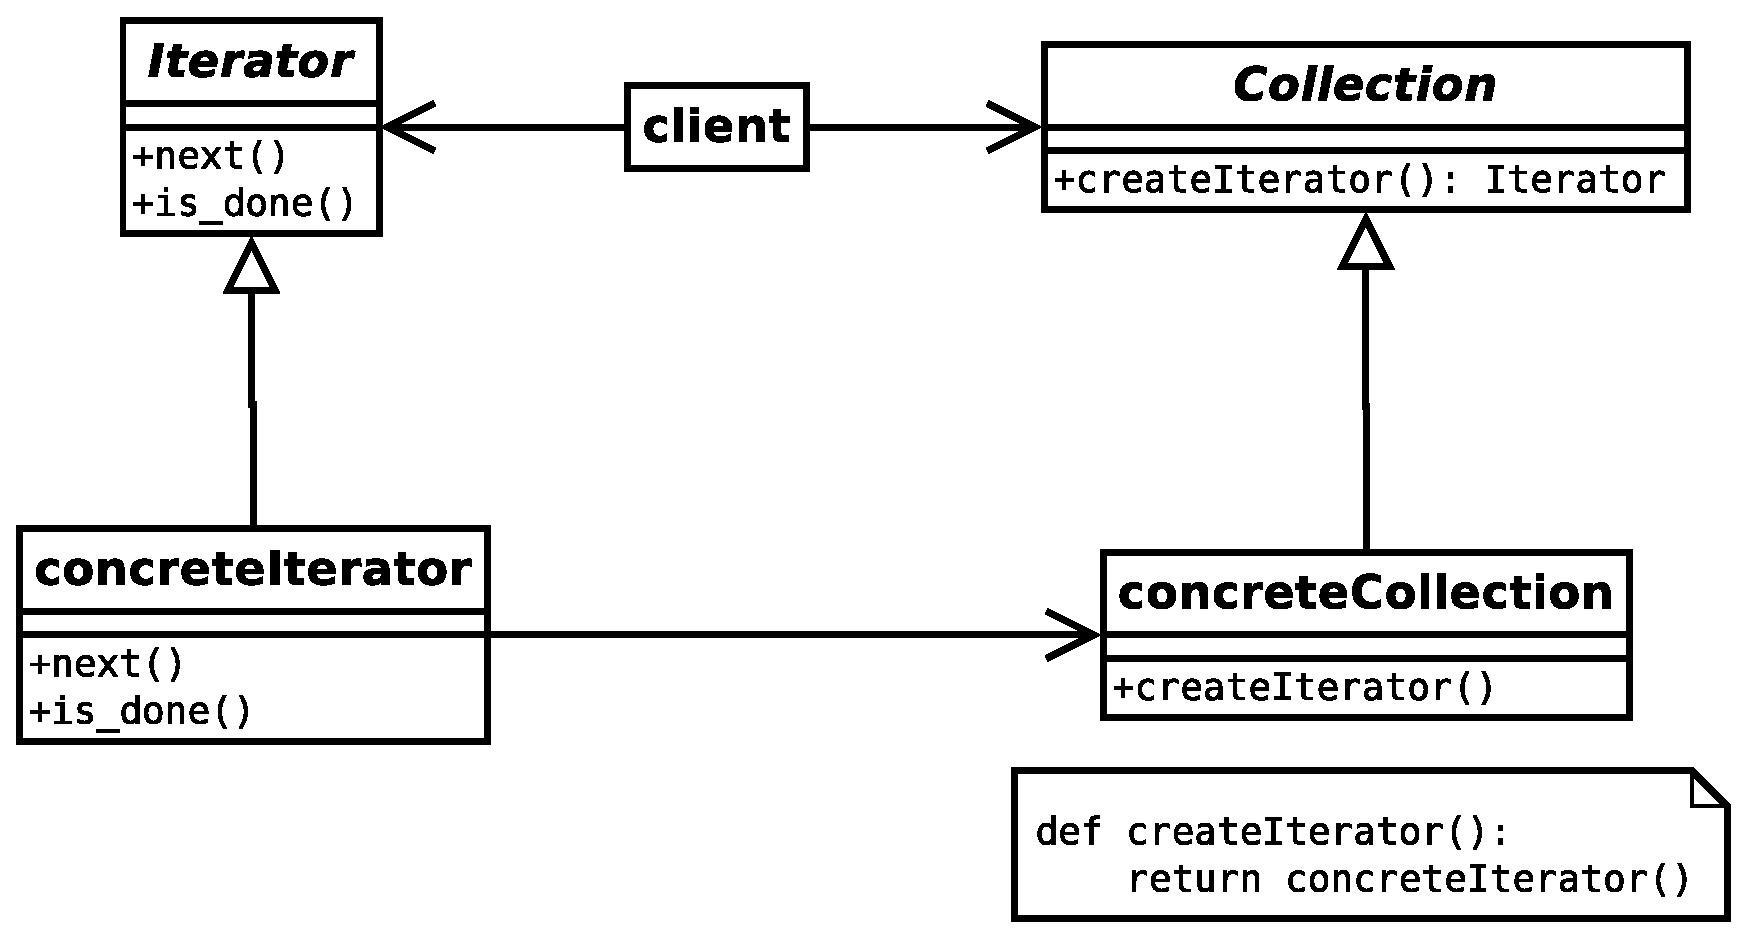
\includegraphics[width=0.75\textwidth]
    {../../diagrams/iterator_pattern.png}
  \caption{ Containers implement the Iterator pattern to allow sequential %
            access to items. }
  \label{fig:iterator_pattern}
\end{figure}


Python helps us create iterator objects by providing an Iterator protocol. In
Python, classes that define the \xfmethod{\_\_iter\_\_()} method can return an
iterator object.  The iterator object needs to define the \xfmethod{next()}
method, which provides the caller an element from the collection being iterated
over. The \xfclass{Container} class, \xfclass{ToolsList}, can act as an
iterator by defining the \xfmethod{\_\_iter\_\_()} and \xfmethod{next()}
methods. The only extra bit it needs to do is to keep track of the current
item, which it does through the \xfparameter{\_\_current\_item} variable, shown
in \Cref{lst:toolslist_iterator}.


\begin{xcode}{%
  language=Python,%
  label=lst:toolslist_iterator,%
  caption={The \xfclass{Container} class implements the Iterator pattern %
           to provide sequential access to items.}%
}
def Container(BasePageWidget):
    ...
    def __iter__(self):
        self.__current_item = 0
        return self

    def next(self):
        ...
        self.__current_item += 1

        if self.__current_item >= self__num_items:
            # reset our counter, stop iterating
            self.__current_item = 0
            raise StopIteration

        return self.get_item_by_position(self.__current_item)
\end{xcode}

The last task of a \xfclass{Container} class is to provide a way to search the
list for items that match some criteria. Two popular ways to access items from
the container are by position and by property.  The type of item returned by the
search methods is tied to the container returning it.  For example, a container
designed to represent a HUBzero support ticket list will return support ticket
list items and a container designed to represent a HUBzero group list will
return group list items.

To keep the \xfclass{Container} class generic, it implements the Factory Method
pattern, allowing subclasses to define which \xfclass{Item} class to
instantiate.

The Factory Method Pattern is used when we want to define an interface for
creating an object, but don't know which class to instantiate. Instead of
always instantiating the same class, we delegate the responsibility to a
subclass.

\begin{figure}[tbh]
  \centering
  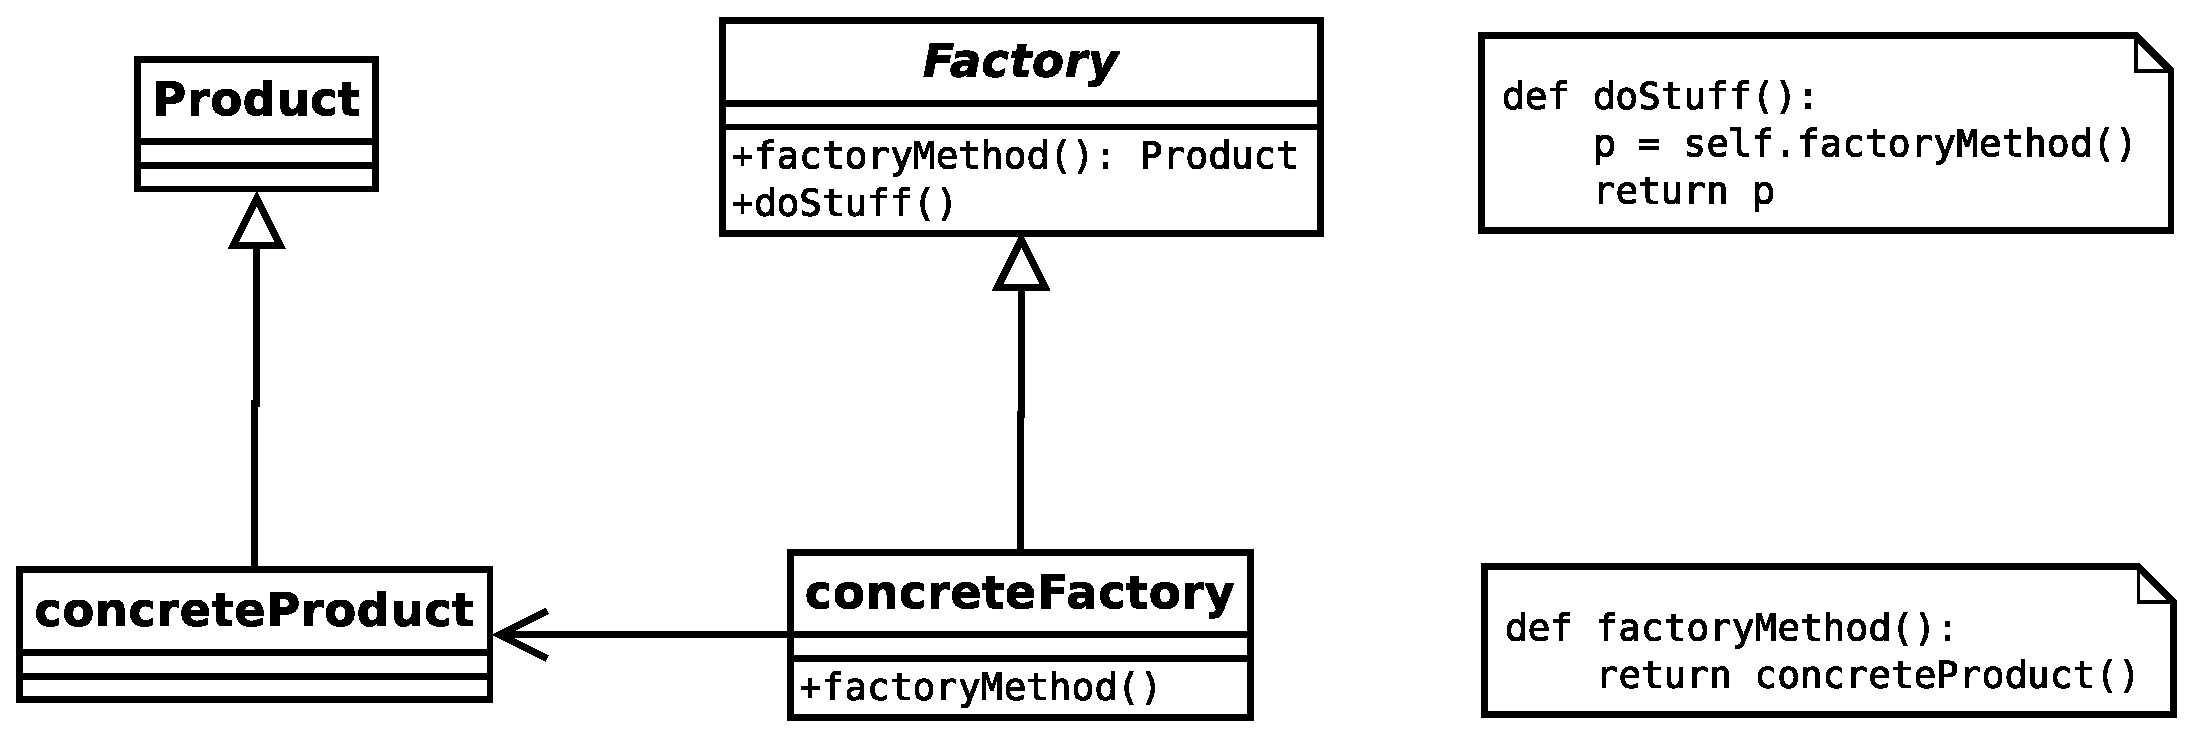
\includegraphics[width=0.75\textwidth]
    {../../diagrams/factory_method_pattern.png}
  \caption{ Containers use the Factory Method pattern to allow derived %
            classes determine the type of Item class to return from searches. }
  \label{fig:factory_method_pattern}
\end{figure}

In the case of the \xfclass{Container} class and the Tool Pipeline example, to
be able to return \xfclass{ToolsItem} objects from searches the
\xfclass{ToolsList} object must know how to create them. The \xfclass{Item}
class and parameters to create an object are saved by the derived container,
and then used by the search methods to instantiate the correct \xfclass{Item}
objects for the container.

\begin{xcode}{%
  language=Python,%
  label=lst:toolslist_constructor,%
  caption={The \xfclass{ToolsList} class manages which type of %
           \xfclass{Item} object to return from searches. In this %
           case \xfclass{ToolsItem} objects.}%
}
class Container(BasePageWidget):
    def __init__(self, owner, locatordict):
        self.item_class = None
        self.item_class_args = None

class ToolsList(Container):
    def __init__(self, owner, locatordict):
        ...
        self.item_class = ToolsItem
        self.item_class_args = [{...}]
\end{xcode}



The \xfclass{ToolsList} class provides two methods for searching through a list
of items.  The first method, \xfmethod{get\_item\_by\_position()}, allows
automation developers to search for an item in the list by position. For
example, developers can ask for the fifth item in the list.
\Cref{lst:toolslist_getitembyposition} shows an implementation of this method
that accepts a counting parameter, \xfparameter{item\_number}, representing the
n-th item in the list. The method uses the \xfclass{Container} object's
\xfclass{Item} class variable, \xfparameter{\_\_item\_class}, to construct the
\xfclass{Item} object for the n-th item in the list.
\xfparameter{\_\_item\_class} uses the \xfclass{Item} class parameters, stored
in \xfparameter{\_\_item\_class\_args}, and the method's
\xfparameter{item\_number} parameter to configure the new page object
representing the specific item.

\begin{xcode}{%
  language=Python,%
  label=lst:toolslist_getitembyposition,%
  caption={The Container class can retrieve Items by position}%
}
    def get_item_by_position(self,item_number):
        result = self.__item_class(
                  self.owner,
                  *self.__item_class_args,
                  item_number=item_number)
        result.detach_from_owner()
        return result
\end{xcode}

The second method, \xfmethod{get\_item\_by\_property()}, allows the developer to search
for the first item in the list that matches a property constraint.  The method
accepts two required parameters, the name of the property and the value it
should match.

\begin{xcode}{%
  language=Python,%
  label=lst:toolslist_getitembyproperty,%
  caption={The Container class can retrieve Items by property}%
}
    def get_item_by_property(self,prop,val):
        result = None

        # create a default item object, using the first item
        r = self.__item_class(self.owner,*self.__item_class_args,item_number=1)
        r.detach_from_owner()

        for item_number in xrange(1,len(items)+1):

            # update the default item object to point to the current item
            r.update_item_number(item_number)

            # check if our current item matches the property constraint
            if r.value()[prop] == val:
              result = r
              break

        # if no items matched, clean up our default item object
        if result is None:
          del r

        return result
\end{xcode}

The \xfmethod{get\_item\_by\_property()} method also uses the
\xfparameter{\_\_item\_class} variable, representing the \xfclass{Item} class,
to construct a new page object that represents a single item in the list.
Similar to the \xfmethod{get\_item\_by\_position()} method, the
\xfmethod{get\_item\_by\_property()} method passes the
\xfparameter{\_\_item\_class}'s constructor a list of arguments to configure
the new page object, including a dictionary of locator templates.

The \xfmethod{get\_item\_by\_property()} method uses an \xfclass{Item} object
to iterate over the items in the list, searching for the first item that
satisfies the property constraint. It takes advantage of the \xfclass{Item}
object's \xfmethod{update\_item\_number()} method and template locators to
update the locators of the object without instantiating a new page object for
each item it encounters in the list. In
\Cref{lst:toolslist_getitembyproperty}, you can see the \xfclass{Item} object
being updated inside of the for loop in line 11, and the comparison between the
item's property and the requested value in line 14.



The ItemList pattern focuses on the interactions of two classes, the
\xfclass{Container} class and the \xfclass{Item} class. In the Tool Pipeline
table example the \xfclass{Container} class, \xfclass{ToolsList}, was
responsible for all of the services provided by the table that were not related
to a specific item or item in the table. The \xfclass{Item} class,
\xfclass{ToolsItem} was responsible for services associated with a specific
item or item in the table.  This separation of services, along with the use of
web element locator templates, allowed the \xfclass{Container} class to
dynamically create page objects for specific items in the table and update the
item being referenced without needing to destroy and create a new object.



\subsection{IframeWrap Pattern}
\label{ssec:iframewrap_pattern}

%
% Used to quickly navigate through layers of iframes to interact with web page
% widgets.

% \subsection{Pattern Name and Classification:}
%
%   IframeWrap Pattern
%   Purpose: Structural - we are defining a good way to dynamically create
%                         a page object to describe and access a specific
%                         item in a list of items.
%   Scope: Object
%

Iframes are another area where using the wrong design can make page objects
difficult to build and inefficient to use and maintain. When hub users upload
resources to a HUBzero website, they are asked to respond to several questions
on a web form, one of which involves describing the resource they are
contributing.  In previous incarnations, the resource contribution form's
description field was a simple HTML <textarea> element. The field handled both
plain text descriptions, but also allowed users to enter a wiki-like markup
language that produced rich text descriptions.  Building a page object with a
<textarea> is pretty rudimentary, and in HUBcheck is represented by the
\xfclass{TextArea} class.


\begin{figure}[tbh]
  \centering
  \includegraphics[width=0.75\textwidth]
    {../../images/hubzero_new_resource_compose_step_abstract_textarea.png}
  \caption{HTML <textarea> based editor. }
  \label{fig:html_textarea_editor_widget}
\end{figure}

\begin{xcode}{%
  language=HTML,%
  label=lst:html_textarea_editor_code,%
  caption={HTML of the textarea based editor.}%
}
<label for="field-fulltxt">
    Abstract/Description:
    <textarea id="field-fulltxt">This is abstract / description text</textarea>
</label>
\end{xcode}

Around the release of version 1.2.0 of the HUBzero software, the web developers
started incorporating a new editor for the description field. Shown in
\Cref{fig:html_iframe_editor_widget}, the new editor incorporated better
controls for handling rich text.  Instead of writing out the wiki syntax to
make words bold, for example, the hub user would press the bold button in the
editor and type the text they wanted to be bold.  This was a great step forward
for usability. The updated editor meant an update was needed for the page
objects that interacted with the previously available <textarea> based editor.
Such a drastic widget change like this usually results in a new page object
being created.



\begin{figure}[tbh]
  \centering
  \includegraphics[width=0.75\textwidth]
    {../../images/mygeohub_new_resource_compose_step_abstract_texteditor.png}
  \caption{HTML iframe based editor.}
  \label{fig:html_iframe_editor_widget}
\end{figure}

\begin{xcode}{%
  language=HTML,%
  label=lst:html_iframe_editor_code,%
  caption={HTML of the iframe based editor, where writing to the %
           <body> tag is just like writing to the %
           <textarea> tag after the automation script %
           enters the iframe.} %
}
<iframe class="cke_wysiwg_frame">
    <html>
        <body class="ckeditor-body">
            <p>This is abstract / description text </p>
        </body>
    </html>
</iframe>
\end{xcode}

Investigating the new web page, one could see that the previous <textarea>
element was replaced with an iframe and embedded web page. Playing around with
the iframe element revealed that once the automation script entered the iframe,
writing text to the <body> element was just like writing text to the <textarea>
element.  This raised the question: \begin{quote}\textit{Do I need to write a
new page object class for an element embedded in an iframe, if a class for that
element already exists and works with the exception of entering and exiting the
iframe?}\end{quote}


\begin{figure}[tbh]
  \centering
  \includegraphics[width=0.50\textwidth]
    {../../images/iframewrap_inputs_example_base.png}
  \caption{Text input fields embedded in different levels of iframes.}
  \label{fig:iframewrap_inputs_example_base}
\end{figure}


Before approaching this question, let's first investigate how iframes work.
\Cref{fig:iframewrap_inputs_example_base} shows an example web page with
some input fields embedded in different levels of iframes.

\begin{figure}[tbh]
  \centering
  \includegraphics[width=0.75\textwidth]
    {../../images/iframewrap_inputs_example_frame_0.png}
  \caption{Text input i0 exists in the default context.}
  \label{fig:iframewrap_inputs_example_frame_0}
\end{figure}

\begin{xcode}{%
  language=HTML,%
  label=lst:html_iframe_example_default_context,%
  caption={In the default context, iframe frame1 references inner\_page.html.}%
}
<html>
    <body>
        <label for="frame1">frame1: </label>
        <iframe id="frame1" src="inner_page.html"></iframe>
        <br/><br/>
        <label for="i0">i0: </label>
        <input type="text" id="i0" value="text input"></input>
    </body>
</html>
\end{xcode}


The first input field, i0, is located in the default context. This is the level
of the web page we generally work in when iframes are not involved.  Along with
the input field i0, this web page also has an iframe, frame1.  In the HTML,
iframes hold the location of another web page to be embedded in the frame. In
this example, frame1 is going to load up the web page inner\_page.html.


\begin{figure}[tbh]
  \centering
  \includegraphics[width=0.75\textwidth]
    {../../images/iframewrap_inputs_example_frame_1.png}
  \caption{Text input i1 exists in the frame1 context.}
  \label{fig:iframewrap_inputs_example_frame_1}
\end{figure}

\begin{xcode}{%
  language=HTML,%
  label=lst:html_iframe_example_frame1_context,%
  caption={inner\_page.html - frame2 references another\_page.html.}%
}
<html>
    <body>
        <label for="frame2">frame2: </label>
        <iframe id="frame2" src="another_page.html"></iframe>
        <br/><br/>
        <label for="i1">i1: </label>
        <input type="text" id="i1" value="my text input"></input>
    </body>
</html>
\end{xcode}

\Cref{fig:iframewrap_inputs_example_frame_1} and
\Cref{lst:html_iframe_example_frame1_context} show the HTML for
inner\_page.html.  It makes up what is referred to as the Frame1 Context. The
Frame1 context has an input field i1, and another iframe, frame2.  Again, the
iframe frame2 holds the location of a web page, and in this case it points to
another\_page.html.


\begin{figure}[tbh]
  \centering
  \includegraphics[width=0.75\textwidth]
    {../../images/iframewrap_inputs_example_frame_2.png}
  \caption{Text input i2 exists in the frame2 context.}
  \label{fig:iframewrap_inputs_example_frame_2}
\end{figure}

\begin{xcode}{%
  language=HTML,%
  label=lst:html_iframe_example_frame2_context,%
  caption={another\_page.html - in frame2 context, only input i2 exists.}%
}
<html>
    <body>
        <label for="i2">i2: </label>
        <input type="text" id="i2" value="my other text input"></input>
    </body>
</html>
\end{xcode}


\Cref{lst:html_iframe_example_frame2_context} shows the HTML for the
file another\_page.html that makes up the Frame2 Context. It contains an input
field i2 that resides within the Frame2 context.


\begin{xcode}{%
  language=Python,%
  label=lst:text_input_field_i0_class,%
  caption={Page object class for i0 text input field.}%
}
class Text(BasePageWidget):
    ...
    # setter
    def value(self, text):
        e = self.find_element(self.locator)
        e.clear()
        e.send_keys(text)
    ...
\end{xcode}

A page object for the i0 input field that resides in the Default Context
would probably include a getter method to retrieve the value of the input, a
setter method to set the value of the input, and maybe an append method to
assist with appending text to whatever was already in the field.  Since the i0
field resides in the default context, there is no need to do anything special;
the methods will find the i0 input element in the HTML DOM, and perform actions
on it.

\begin{xcode}{%
  language=Python,%
  label=lst:text_input_field_i1_class,%
  caption={Page object class for i1 text <input> field.}%
}
class Text1Frame(BasePageWidget):
    ...
    # setter
    def value(self, text):
        frame = self.find_element('#frame1')
        self._browser.switch_to_frame(frame)
        e = self.find_element(self.locator)
        e.clear()
        e.send_keys(text)
        self._browser.switch_to_default_content()
    ...
\end{xcode}

Building a page object for the i1 input field involves a little more work.
The page object is almost the same as the one for the i0 input field, but
because i1 is located inside of the Frame1 context the web browser needs to be
instructed to traverse the frame1 iframe before performing any getter, setter,
or append actions.  So inside each of the page object's methods a few lines of
code need to be added for entering and exiting the iframe. After the web
browser has entered the Frame1 context it can search for the element in the
HTML DOM and perform actions on the element.  In
\Cref{lst:text_input_field_i1_class}, the extra code for entering and exiting
the Frame1 context shows up in lines 5-6 and line 10.  Lines 7-9 make up the
core action of the widget and are the same as what is found in the page object
for text input i0, in \Cref{lst:text_input_field_i0_class}.


\begin{xcode}{%
  language=Python,%
  label=lst:text_input_field_i2_class,%
  caption={Page object class for i2 text input field.}%
}
class Text2Frame(BasePageWidget):
    ...
    # setter
    def value(self, text):
        frame1 = self.find_element('#frame1')
        self._browser.switch_to_frame(frame1)
        frame2 = self.find_element('#frame2')
        self._browser.switch_to_frame(frame2)
        e = self.find_element(self.locator)
        e.clear()
        e.send_keys(text)
        self._browser.switch_to_default_content()
    ...
\end{xcode}

Building a page object for the i2 input field adds another layer of iframe
context traversal.  Remember, i2 is located inside of the Frame2 context, which
is located inside of the Frame1 context. The methods for the i2 page object
have the same core actions as those of the i0 and i1 page objects, but include
code to traverse two iframe contexts. This can be seen in
\Cref{lst:text_input_field_i2_class}, where the setter method first moves from
the Default context to the Frame1 context in lines 5-6, then moves from the
Frame1 to the Frame2 context in lines 7-8. The setter method next performs the
method's core action in lines 9-11 and finally returns back to the default
context in line 12.


To review, building page objects for the i0, i1 and i2 input fields involves
tracking the current frame level and possibly traversing frame levels to be in
the correct context for interacting with an element.  In the example from
\Cref{fig:iframewrap_inputs_example_base}, all of the page objects
started off with the same code, but for input i1, additional lines were added
to account for entering and exiting the Frame1 context.  Similarly, for input
i2, additional lines of code were added to account for entering and exiting the
Frame1 and Frame2 contexts.  But the question remains: \begin{quote}\textit{Is there a way
to handle the entering and exiting of iframes outside of the page object so we
can reuse our original page object that represents a Text <input> field on a
web page?}\end{quote}

In essence, a solution would provide a way to write the core methods of a page
object once and if the page object was found inside of an iframe, the methods
could be wrapped with code to enter and exit the iframe. If the page object was
found inside of two, or three, or more iframes, the methods would just keep
getting wrapped with code to enter and exit iframe contexts.


\begin{figure}[tbh]
  \centering
  \includegraphics[width=0.75\textwidth]
    {../../images/iframewrap_pattern_multiple_frames.png}
  \caption{IframeWrap pattern wraps the core of methods with code to %
           traverse iframe contexts.}
  \label{fig:iframewrap_pattern_multiple_frames}
\end{figure}


This is the idea behind the IframeWrap pattern. It uses the Decorator pattern
to \textit{decorate} or wrap the attributes of a page object with code to enter
an iframe context, call the original page object method, and then exit the
iframe context. It supports both page objects from the default context as well
as previously wrapped page objects.


\begin{figure}[tbh]
  \centering
  \includegraphics[width=0.75\textwidth]
    {../../images/decorator_pattern_before_after.png}
  \caption{Decorator pattern}
  \label{fig:decorator_pattern}
\end{figure}


The purpose of the Decorator pattern is to extend functionality of an object
without necessarily changing the interface. It is most often used when a
specific object needs to be changed at runtime without affecting other objects
of the class.  It does this by wrapping the original functionality of the
object's attributes with code to do extra work.

Consider the example object \xfobject{a} shown in \Cref{fig:decorator_pattern},
which is an instance of the class \xfclass{A}, with a method \xfmethod{f}.
Additional responsibilities can be added to \xfobject{a}'s method \xfmethod{f}
by first pointing \xfparameter{a.f} to a wrapper method and then directing the
wrapper method to perform the extra work and call the method that
\xfparameter{a.f} used to point to.

\begin{figure}[tbh]
  \centering
  \includegraphics[width=0.75\textwidth]
    {../../images/decorator_pattern_applied_to_i1.png}
  \caption{Decorator pattern applied to text input field i1 in Frame1 context}
  \label{fig:decorator_pattern_i1}
\end{figure}


The same idea can be applied to the \xfclass{Text} page object, from
\Cref{lst:text_input_field_i0_class}, to create a page object for the i1 input
in the Frame1 context. The page object's \xfmethod{value()} method performs the
core actions for setting or getting the value of the underlying HTML element.
In Python, \xfmethod{value()} is an attribute that points to a function object,
which can be decorated to add the enter and exit iframe commands.  After
decorating the function object, the value attribute will point to a wrapper
function that enters the correct iframe context, calls the original function
object, and returns back to the default context.


\begin{xcode}{%
  language=Python,%
  label=lst:iframewrap_example_po,%
  caption={Page object class for web page with multiple text input field %
           embedded in frames.}%
}
class FramedInputs(BasePageObject):
    def __init__(self):
        self.i0 = Text('#i0')
        self.i1 = IframeWrap( Text('#i1'), ['#frame1'] )
        self.i2 = IframeWrap( Text('#i2'), ['#frame2', '#frame1'] )
\end{xcode}

A page object class that represents the web page shown in
\Cref{fig:iframewrap_inputs_example_base} can be built by instantiating and
decorating the \xfclass{Text} class from \Cref{lst:text_input_field_i0_class}.
In \Cref{lst:iframewrap_example_po}, the variable self.i0 instantiates a
\xfclass{Text} object to represent the text input field in the default context.
The variables self.i1 and self.i2 also instantiate \xfclass{Text} objects, but
immediately passes them to the \xfmethod{IframeWrap()} function. The
\xfmethod{IframeWrap()} function accepts a page object and a list of locators
for frames that must be traversed to access the element represented by the page
object. For example, the i1 text input field resides within a frame with a
locator \xflocator{\#frame1}, so the \xfmethod{IframeWrap()} function is sent
the single element list \xfinlinecode{['\#frame1']}.  Similarly, the i2 text
input field resides in a frame with a locator \xflocator{\#frame2}, which
itself resides in a frame with a locator \xflocator{\#frame1}, so the
\xfmethod{IframeWrap()} function is sent a two element list containing both
locators.


\begin{xcode}{%
  language=Python,%
  label=lst:iframetracker_class,%
  caption={\xfclass{IframeTracker} objects manage wrapping object methods %
           and attributes}%
}
class IframeTracker(object):
    ...
    def wrap_callable_attributes(self,o):
        for attr, item in o.__class__.__dict__.items():
            if callable(item):
                item = getattr(o,attr)
                setattr(o,attr,self.wrap_attribute(item))

    def wrap_attribute(self,item):
        def wrapper(*args, **kwargs):
            ...
            switched = self._switch_to_iframe_context(final_framelevel)
            result = item(*args, **kwargs)
            self._switch_to_iframe_context(initial_framelevel)
            return result
        return wrapper
\end{xcode}



Internally, the \xfmethod{IframeWrap()} function creates an
\xfclass{IframeTracker} object and associates it with the page object that is
to be decorated. The \xfclass{IframeTracker} object is responsible for tracking
frame levels and wrapping the object's attributes.  The most interesting part
of the \xfclass{IframeTracker} object is when the page object gets decorated,
which is shown in \Cref{lst:iframetracker_class}.  First the
\xfmethod{IframeWrap()} method calls the
\xfmethod{wrap\_callable\_attributes()} method, which identifies callable
attributes from the object, including methods. Within the page object, the
callable attribute is replaced with a call to the \xfmethod{wrapper()} method,
which is a closure that stores the function object it replaces.  Just as shown
in \Cref{fig:decorator_pattern}, the \xfmethod{wrapper()} method takes
care of entering the correct frame context, calling the original method it
replaces that performs the core actions, and returning back to the original
frame context.


\begin{xcode}{%
  language=Python,%
  label=lst:iframewrapd_po_use,%
  caption={IframeWrap'd page objects work just like non-wrapped page objects.}%
}
class FramedInputs(BasePageObject):
    def __init__(self):
        self.i0 = Text('#i0')
        self.i1 = IframeWrap( Text('#i1'), ['#frame1'] )
        self.i2 = IframeWrap( Text('#i2'), ['#frame2', '#frame1'] )


po = FramedInputs()

# print out the current text in the widgets
print "i0.value = %s" % (po.i0.value)
print "i1.value = %s" % (po.i1.value)
print "i2.value = %s" % (po.i2.value)

# update the text in the widgets
po.i0.value = 'i0 text'
po.i1.value = 'new i1 text'
po.i2.value = 'new i2 text too'
\end{xcode}


With the page object attribute wrapping process complete, the newly
IframeWrap'd page object is ready for use. Inside of automation scripts, the
decorated page objects work just like the non-decorated page objects. The
automation developer doesn't need to do anything special to access or interact
with the wrapped page objects. In \Cref{lst:iframewrapd_po_use}, the variables
i0, i1, and i2 are all accessed from the page object po in the same way.  The
responsibility for managing the frame traversal has been embedded within the
page object. The difference between text input field page objects is only
exposed in how the page objects are instantiated.

When implementing the IframeWrap pattern in Python there are a few gotchas. Not
all page object attributes need to be wrapped. Some attributes do not try to
interact with the web element the page object represents. Keeping a list of
these attributes is handy so the wrapping of these attributes can be skipped.
Additionally wrapping Python object properties can be tricky because properties
are a part of the class, not the object. It requires creating a new class
object from the page object's class, decorating the properties of the new class
object, and associating the page object with the new class.



\section{Summary of Page Object Based Design Patterns}
\label{sec:summary_page_object_design_pattern}

The Page Object design pattern provides developers with an object-oriented way
to think about dissecting web pages. Its framework for creating reusable pieces
of code to represent parts of web pages can simplify the process of building
robust web automation software, but sometimes taking a naive approach can lead
to an inefficient page object design. In this chapter, we saw three situations
where implementing a naive page object design could lead to inefficient
programs. Instead, more robust designs were offered as solutions which helped
increase code reuse.

The first situation involved the frequent situation of building page objects
for web forms.  Due to similarities in the design and goals of web forms, we were
able to reduce their use to answering questions, filling the answers into fields
on the web page, and pressing the submit or cancel button. This generalization of
goals allowed us to recognize that with the exception of the specific fields
that needed to be populated, a large portion of building page objects for web
forms could be abstracted into a generic \xfclass{Form} superclass. Fields
could then be specified in a derived subclass.

In the second case we investigated building page objects for lists of items on
a web page where there is no a priori knowledge of the number of items
displayed.  The ItemList Pattern encourages users to build a single page object
to represent an item in a list, and update which item in the list the page
object points to instead of trying to build a separate class for each item in
the list.

Lastly, we considered building page objects for web page elements that exist in
different iframe levels. While it may be tempting to manually create a new page
object class for an element that exists in an iframe, this approach discourages
code reuse. Instead, the IframeWrap pattern decorates a page object's
attributes with additional code to enter and exit the proper iframe context
without changing the original object's interface.
